\chapter{Methodology}

\section{Overview}

In this section, we can see the details of the approach taken to design and implement the JSONPath parser. It includes the system architecture, parsing techniques, grammar design, implementation details, error handling strategies, and testing methodology.

\section{System Architecture}

The JSONPath parser system is built with some many key components:

\begin{itemize}
	\item \textbf{Lexer (Tokenizer)}: Converts the input JSONPath query string into a stream of tokens like identifiers, operators, brackets, and literals.
	\item \textbf{Parser}: Processes the token stream according to the JSONPath grammar to build a parse tree representing the query structure.
	\item \textbf{Evaluator}: Traverses the parse tree to evaluate the query against input JSON data, retrieving the requested nodes or values.
	\item \textbf{Error Handler}: Find out and reports syntax errors in the JSONPath expressions, giving meaningful feedback to the user.
\end{itemize}

\section{Parsing Approach}

The parser is developed using a \textbf{recursive descent parsing} technique due to JSONPath’s relatively straightforward and context-free grammar. This approach used for clear, modular parsing functions for each grammar rule, making the parser easier to maintain and extend.

Moreover, parser generators such as Bison and Flex could be used to implement an LR parser; however, recursive descent was chosen for its simplicity and flexibility in handling filters and expressions within JSONPath.

\section{Grammar Design}

The grammar of JSONPath was adapted from the IETF JSONPath specification (RFC 9535) and existing implementations such as PostgreSQL’s \texttt{jsonpath\_gram.y}. Impotent grammar rules are following:

\begin{itemize}
	\item \textbf{Root Selector}: The starting point symbol \texttt{\$}.
	\item \textbf{Child and Recursive Descent}: Operators \texttt{.} and \texttt{..} select child nodes or recursively descend into nested structures.
	\item \textbf{Array Indexing and Slicing}: Square brackets \texttt{[ ]} used to select array elements by index or slices.
	\item \textbf{Filters}: Expressions inside \texttt{[?()]} gives conditional selection according on logical and comparison operators.
\end{itemize}

The grammar was built in a modular manner, with separate parsing functions handling selectors, filters, expressions, and literals.

\section{Implementation Details}

The parser is developed with \textbf{C++} (or specify your language) using modern programming. necessary tools and libraries include:

\begin{itemize}
	\item \textbf{Lexer}: A hand-written tokenizer that reads input character-by-character to generate tokens.
	\item \textbf{Parser}: Recursive descent functions developed manually without parser generator tools.
	\item \textbf{JSON Library}: make practical and effective use of a third-party JSON library such as \texttt{nlohmann/json} for parsing and manipulating input JSON data.
	\item \textbf{Development Environment}: Built and tested using \texttt{g++} compiler on Linux, with \texttt{CMake} for build automation.
\end{itemize}
\begin{figure}[htbp]
	\centering
	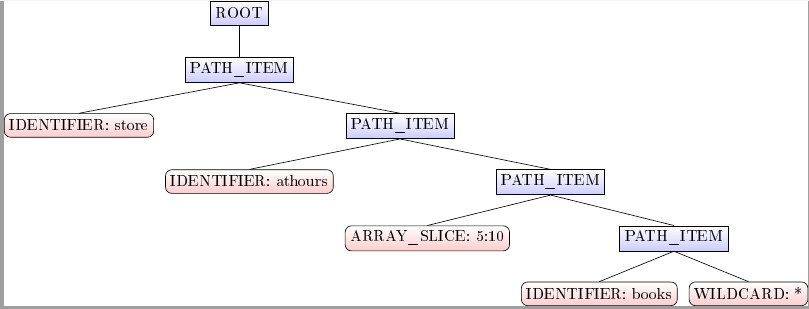
\includegraphics[width=0.7\textwidth]{images/op_graph.png}
	\caption{Sample output of the JSONPath parser evaluating a query on test JSON data.}
	\label{fig:parser_output}
\end{figure}

\section{Integration with YottaDB Query}

To add the functionality in the JSONPath parser, the parsed queries are compiled into YottaDB query language statements. This gives seamless querying of JSON-like hierarchical data stored in the YottaDB database.

The compilation process converts JSONPath expressions such as property selectors, filters, and array indexing into equivalent YottaDB query commands, allow execution of query within the database environment.

Figure~\ref{fig:yottadb_output} shows a sample output of a compiled JSONPath query executed on YottaDB data.

\begin{figure}[htbp]
	\centering
	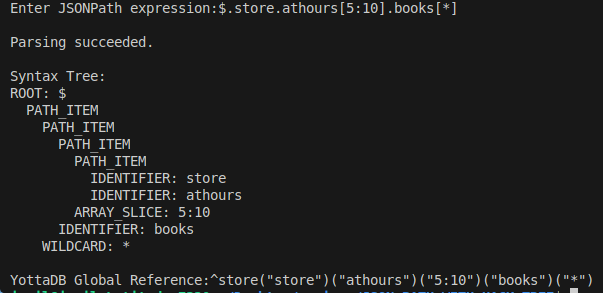
\includegraphics[width=0.7\textwidth]{images/yottadb_output.png}
	\caption{Output of the JSONPath query compiled and executed as a YottaDB query.}
	\label{fig:yottadb_output}
\end{figure}

\section{Error Handling}

The parser includes error detection to handle:

\begin{itemize}
	\item \textbf{Syntax Errors}: Missing brackets, invalid tokens, or unexpected symbols in JSONPath expressions are reported with descriptive error messages.
	\item \textbf{Semantic Errors}: Wrong filter expressions or unsupported operations gives errors.
\end{itemize}

Error handling allows the parser to terminate when it needed or used for limited recovery where possible, improving user experience.

\section{Testing and Validation}

To make sure parser is correct and robust or not, it was tested using:

\begin{itemize}
	\item \textbf{Unit Tests}: Cover individual parser functions and lexer components, including edge cases.
	\item \textbf{Test JSON Datasets}: Sample JSON documents representing various complexities and structures.
	\item \textbf{Query Samples}: JSONPath queries starting from simple property access to complex filtered expressions.
\end{itemize}


\section{Limitations}

The current implementation contains most standard JSONPath features but some advanced functions like regular expression matching or user-defined functions are not supported yet, but future work can extend support for these features and improving error recovery.

